\section{Performance Evaluation} \label{sec:eval}

We used two platforms to evaluate the performance of \textit{PackDrop}:

\begin{itemize}
	\item \textbf{Platform 1:} A cluster called \textit{Graphene} from \textit{Grid'5000} with $4$ PEs per node and  a Gigabit Ethernet interconnection network.
	\item \textbf{Platform 2:} A subset of a tightly coupled supercomputer called \textit{Santos Dumont} from the Brazilian National Laboratory for Scientific Computing (LNCC) with $24$ PEs per node and an Infiniband interconnection network.% supported by Intel's Parallel Studio XE implementation of \texttt{MPI} (v2017.4).
\end{itemize}

All applications were compiled with {\small\texttt{gcc}} with the following flags: {\small\texttt{-std=c++11 -O3}}. Details of both platforms are available on Table~\ref{tab:ptinfo}.

\begin{table}[t]
    \centering
    	\caption{Overview of the experimental platforms.}
	\begin{tabular}{lll}
	\toprule
	\textbf{Characteristics}	& \textbf{Platform 1} 		& \textbf{Platform 2}	\\
	\midrule
		\# of nodes	   		& 32 					& 16 -- 32 \\
        \# of CPUs/node	   	& $4$ (UMA) 				& $2\times12$ (NUMA) \\
        CPU Model			& Intel Xeon X3440 		& Intel Xeon E5-2695v2 \\
        CPU Freq.  			& $2.53$GHz				& $2.4$GHz \\
        RAM/node    			& $16$GB					& $64$GB	 \\
        Network 				& Gigabit Ethernet		& Infiniband FDR \\
        OS      				& Ubuntu 14.04			& RedHat Linux 6.4 \\
        GCC	version			& $5.4.0$				& $5.3.1$	\\
        Charm++ version		& $6.8.1$				& $6.8.1$ 	\\
        Communication		& UDP					& MPI $3.1.0$	\\
        \bottomrule
	\end{tabular}
    \label{tab:ptinfo}
\end{table}

In the next sections we present the metrics used to compare \packdrop with \greedylb, \refinelb, \distributedlb and \dummylb.
Then, we discuss the results obtained in both platforms presented in Table~\ref{tab:ptinfo} and the scalability of \packdrop.
All raw data of our results, as well as parsing scripts for analysis are publicly available\footnote{Available at: \texttt{https://github.com/eclufsc/\\packdrop-data-analysis}}.

\subsection{Metrics}

\textit{Application time} (makespan) is one of the most relevant metrics to evaluate load balancers in \charm.
Since migrations may induce high overheads and could impact communication costs, a bad load balancing strategy algorithm may present fast decision times but it may increase load imbalance considerably. Thus, the overall execution time of the application will also be increased.
This is a powerful metric to measure both load balancing precision and the overall impact of the strategy on parallel applications.

\textit{Load balancer decision time}, on the other hand, is an indicator of its scalability.
Some centralized schedulers, such as \greedylb, work very well on local machines, with a reasonable data input.
However, when executing on distributed memory environments, the scalability of centralized strategies is limited due to their high decision time in these scenarios.
Throughout this section, load balancer decision time will also be referred to as \textit{rescheduling time}.

\subsection{Evaluation on Platform 1} \label{sec:cluster}

All experiments executed on Platform 1 were compiled with \charm using the {\small\texttt{--with-production}} option, combined with the specifications detailed on Table~\ref{tab:ptinfo}.
Overall, $32$ homogeneous compute nodes were used, with a total of $128$ PEs.

\subsubsection{Evaluation with Synthetic Load} \label{sec:cluster:lbtest}

\textit{LB Test} experiments had a total of $18,990$ \textit{tasks}, executed over $150$ iterations, performing load balance every $40$ iterations.
\textit{Task} loads varied from $30$ms to $9000$ms, which provides reasonable load imbalance, causing global rescheduling to be useful in this case.
Ring, $2$D mesh and $3$D mesh communication topologies were used to provide different levels of migration impact and communication costs.

%\todo[inline]{Figure~\ref{fig:eval:g5k:lbtest:apptime} and Table~\ref{tab:lbtest:apptime} present the \textbf{very same result}. The same observation holds for Table~\ref{tab:eval:g5k:leanmd:time} and in Figure~\ref{fig:eval:g5k:leanmd:time}. You should either use tables or the figures. If you put both, it seems to me that you're trying to ``encher linguiça''.}

\begin{table}[h]
	\centering
    \caption{Average application time for \textit{LB Test} on Platform 1.}
	\begin{tabular}{l  c  c  c}
    \toprule
	\multirow{2}{*}{\textbf{Scheduler}} 	& \multicolumn{3}{c}{\textbf{Network Topologies}} \\ \cmidrule{2-4}
 								& Ring & Mesh2D & Mesh3D \\
	\midrule
        \distributedlb 		& $47.493$s & $48.648$s & $49.055$s \\
        \greedylb 			& $46.541$s & $49.560$s & $51.068$s \\
        \dummylb 			& $52.430$s & $53.172$s & $53.941$s \\
        \packdrop 			& $46.816$s & $47.371$s & $47.974$s \\
        \refinelb 			& $45.491$s & $46.293$s & $47.219$s \\
        \bottomrule
	\end{tabular}
    \label{tab:lbtest:apptime}
\end{table}

%\begin{figure}
%	\centering
%	\subfigure[LB Test]{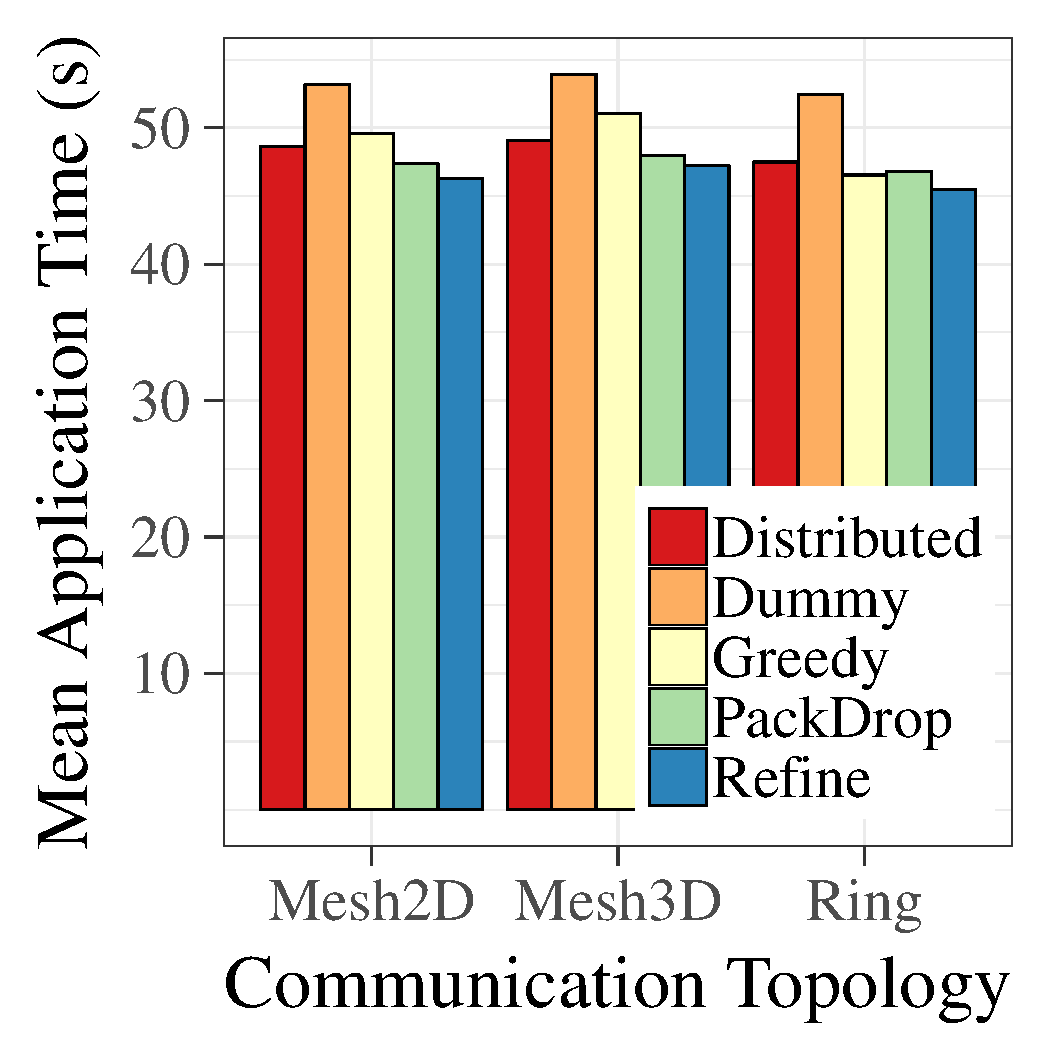
\includegraphics[width=0.45\linewidth]{images/apptime_lbtest_g5k.pdf}\label{fig:eval:g5k:lbtest:apptime}}	
%	\subfigure[LeanMD]{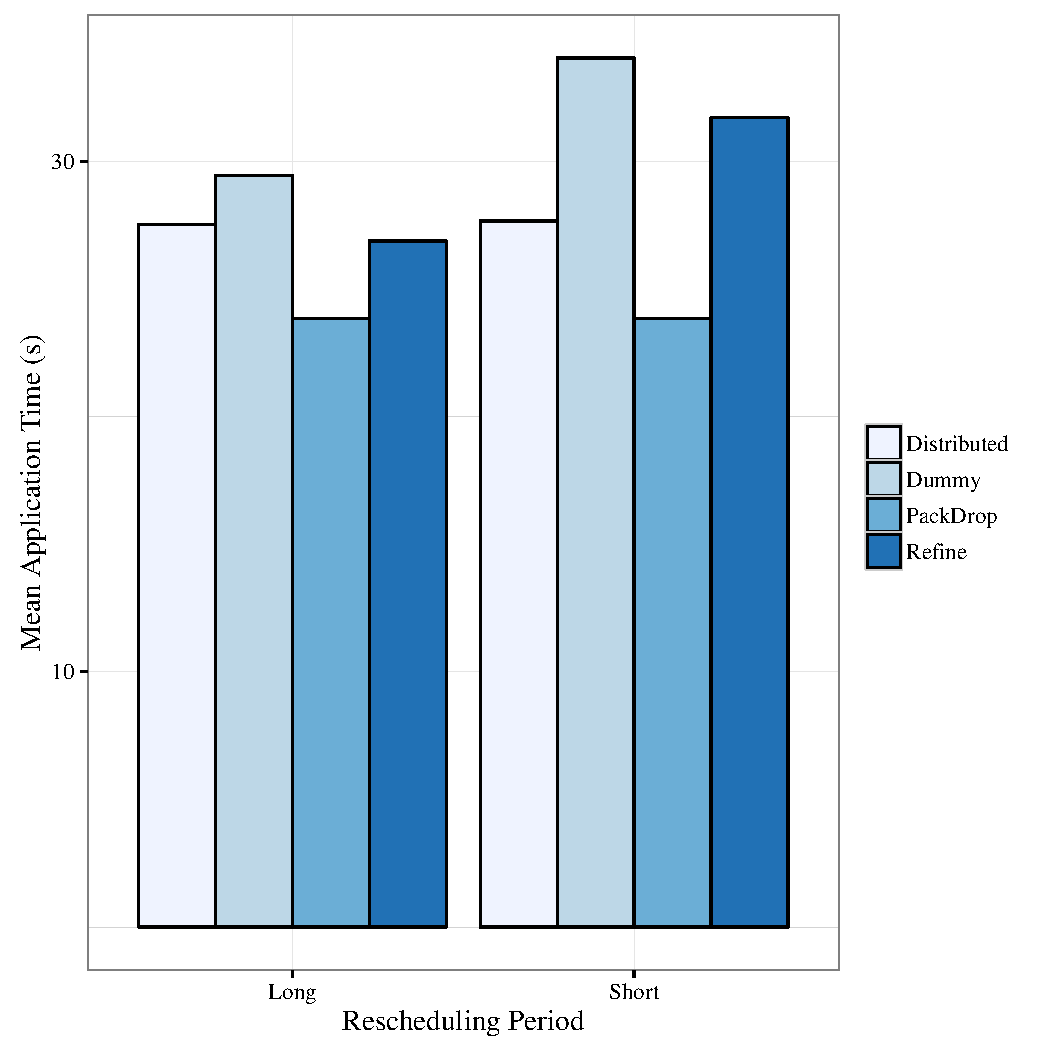
\includegraphics[width=0.45\linewidth]{images/apptime_leanmd_g5k.pdf}\label{fig:eval:g5k:leanmd:time}}
%	\caption{Cluster Execution Results for both applications.}
%	\label{fofinho3}
%\end{figure}

%\todo[inline]{Análise estatística para poder dizer que esses tempos são verdadeiramente diferentes?}

Each configuration of the benchmark was executed $15$ times, with results depicted in Table~\ref{tab:lbtest:apptime}.
Observed application times present a maximum $2\%$ standard deviation from the mean. 
Results for \greedylb show how different communication topologies affect the scheduling performance.
Since \greedylb migrates many \textit{tasks}, the more they communicate, the more migrations impact the application time.

The increased in communication cost can be verified among all scheduling strategies, but in none as much as in \greedylb.
Our novel approach (\packdrop) has outperformed the other decentralized strategy (\distributedlb) in the \textit{LB Test} case in this scale.
However, since the platform is not large enough to present all of the potential gains of decentralized strategies, \refinelb still outperformed any other scheduler in this benchmark.
Nevertheless, this indicates a good scalability potential for \packdrop, specially in a cluster with high communication overhead due to its Gigabit Ethernet connection. %interconnection?

\subsubsection{Evaluation with Molecular Dynamics} \label{sec:cluster:md}

\textit{LeanMD} experiments generated a $9\times9\times9$ space, with a total of $27,702$ \textit{tasks}.
Each execution ran $500$ iterations, with a first rescheduling step at the $10$th iteration. 
Rescheduling periods (RP) of every $30$ (short) and every $60$ (long) iterations were used, providing different impacts of rescheduling on the application.
\greedylb and \dummylb were excluded from this evaluation due to their high cost in an application such as \textit{LeanMD}. 

\begin{table}[!ht]
	\centering
	\caption{Average application time for \textit{LeanMD} on Platform 1.}	
	\begin{tabular}{l c c c}
	\toprule
	%\textbf{Scheduler} & Time (Short RP) & Time (Long RP) & Mean LB Time \\ 
	\multirow{2}{*}{\textbf{Scheduler}} 	& \multicolumn{2}{c}{\textbf{Rescheduling Period}} & \multirow{2}{*}{\textbf{Rescheduling Time}} \\ \cmidrule{2-3}
 								& Short & Long \\	
	\midrule
	
	\distributedlb & $69.356$s & $68.360$s & $167.044$ms \\ 
	\packdrop & $55.984$s & $55.516$s & $143.103$ms \\ 
	\refinelb & $59.357$s & $55.899$s & $539.836$ms \\ 
	\bottomrule	
	\end{tabular}
	\label{tab:eval:g5k:leanmd:time} 
\end{table}

%\begin{figure}[!ht]
%	\centering
%    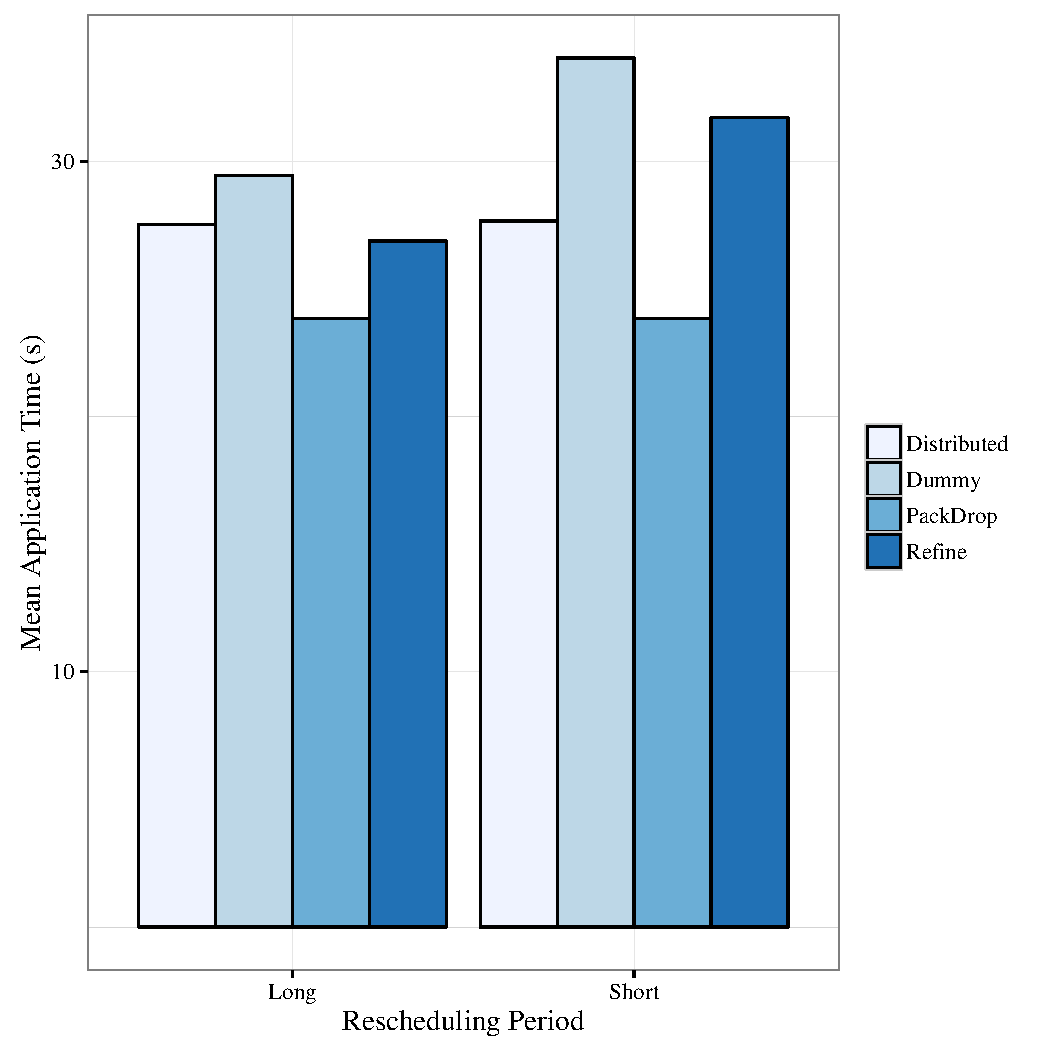
\includegraphics[width=0.43\textwidth]{images/apptime_leanmd_g5k.pdf}
%	\caption{LeanMD cluster execution results.}
%    \label{fig:eval:g5k:leanmd:time}
%\end{figure}

%\todo[inline]{Não acho que precisamos da figura dos tempos de escalonamento.}

%\begin{figure}[!t]
%	\centering
%    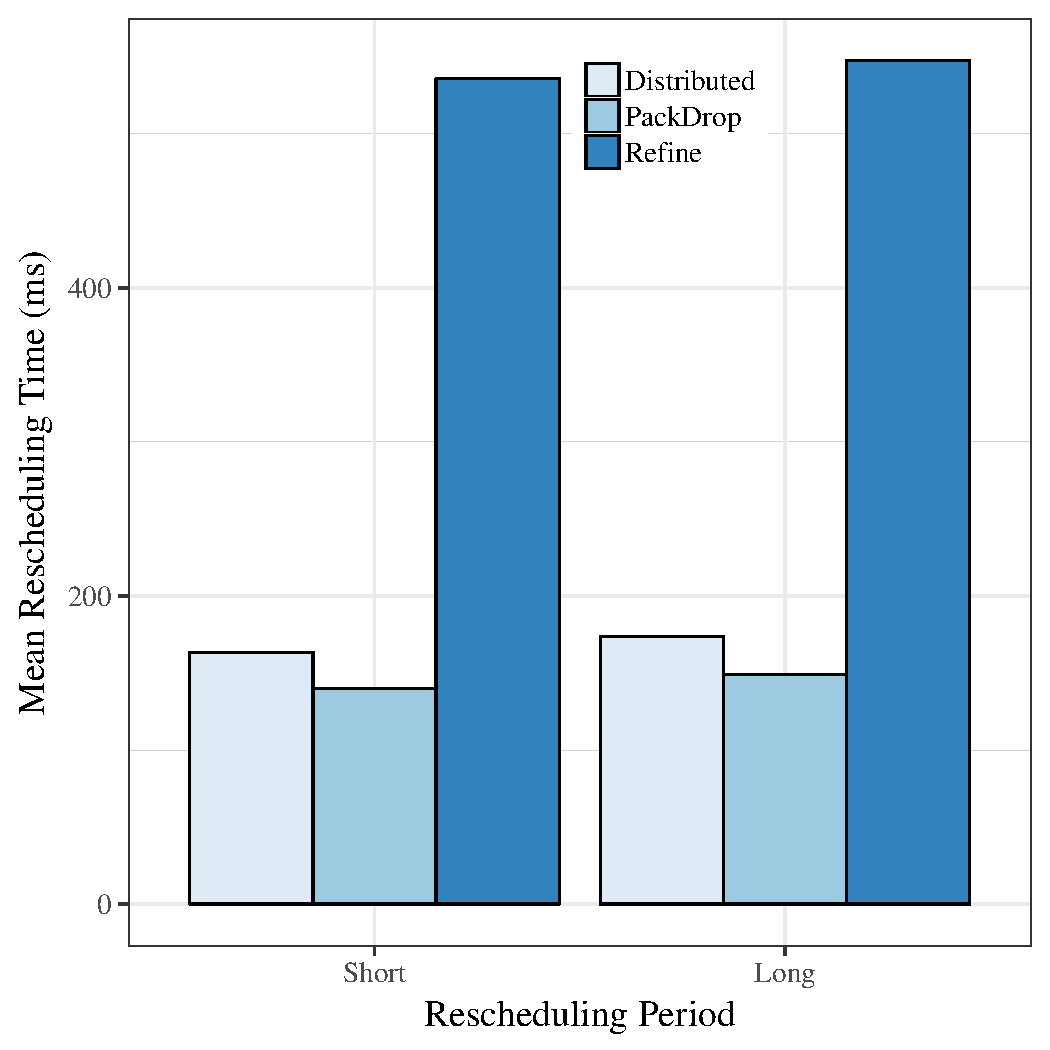
\includegraphics[width=0.43\textwidth]{images/schedtime_leanmd_g5k.pdf}
%	\caption{LeanMD cluster execution results.}
%    \label{fig:eval:g5k:leanmd:schedtime}
%\end{figure}

Each configuration of \textit{LeanMD} was executed $10$ times, making a total of $5,000$ steps per configuration and are depicted in Table~\ref{tab:eval:g5k:leanmd:time}.
Observed application times presented a standard deviation from the mean lower than $2\%$ for all results presented.

Results show a better overall performance of \packdrop, outperforming the other strategies in the two scenarios chosen.
Since our strategy migrates groups of tasks, it preserves locality of tasks after migration. 
Because of that, it was able to outperform \distributedlb.

The \textit{Rescheduling Time}, presented in Table~\ref{tab:eval:g5k:leanmd:time}, shows the time taken by the periodical rescheduling (LB), task migration and the first iteration after the LB call.
It shows the increased cost of \refinelb, which is due to both information aggregation costs and dealing with the high amounts of application data in a centralized fashion.
\packdrop displays its effectiveness in rescheduling time, outperforming the other strategies and resulting in an overall better application time. 

\subsection{Evaluation on Platform 2} \label{sec:sdumont}

All experiments executed on Platform 2 were compiled with \charm using the {\small\texttt{--with-production}} option, combined with the specifications detailed on Table~\ref{tab:ptinfo}.
Different numbers of homogeneous $2\times 12$ PEs compute nodes ($2$ NUMA-nodes with $12$ cores each) were used to evaluate the scalability of \packdrop.
We ranged from $16$ ($384$ PEs) to $32$ ($768$ PEs) unique nodes in our evaluation. 

\subsubsection{Evaluation with Molecular Dynamics} \label{sec:sdumont:md}

\textit{LeanMD} experiments generated a $10\times15\times10$ space, with a total of $171$K \textit{tasks}.
Each execution ran $100$ iterations, with a first rescheduling step at the $9$th iteration. 
Rescheduling was performed every $30$ iterations and each configuration of \textit{LeanMD} was executed $10$ times, making a total of $1,000$ steps per configuration. 

%\begin{table}
%	\centering
%	\caption{LeanMD Supercomputer Results.}
%	\begin{table}{l|c|c}
%	Scheduler 	& Application Time 	& LB Time \\ \hline
%	Dummy 		& $59.35696$s 		& $539.8364$ms \\ 
%	Greedy 		& 					& \\
%	Distributed	& $69.35606$s  		& $167.0444$ms \\ 
%	PackDrop 	& $55.98428$s 		& $143.1028$ms \\ 
%	
%	\end{table}
%	\label{tab:eval:sdumont:leanmd}
%\end{table}

%\todo[inline]{Log times option added. If we keep the log option on resched time, it is possible to portray Refine results in a satisfatory way.}

\begin{figure}[!ht]
 \centering
 \subfigure[Application Time (s).]{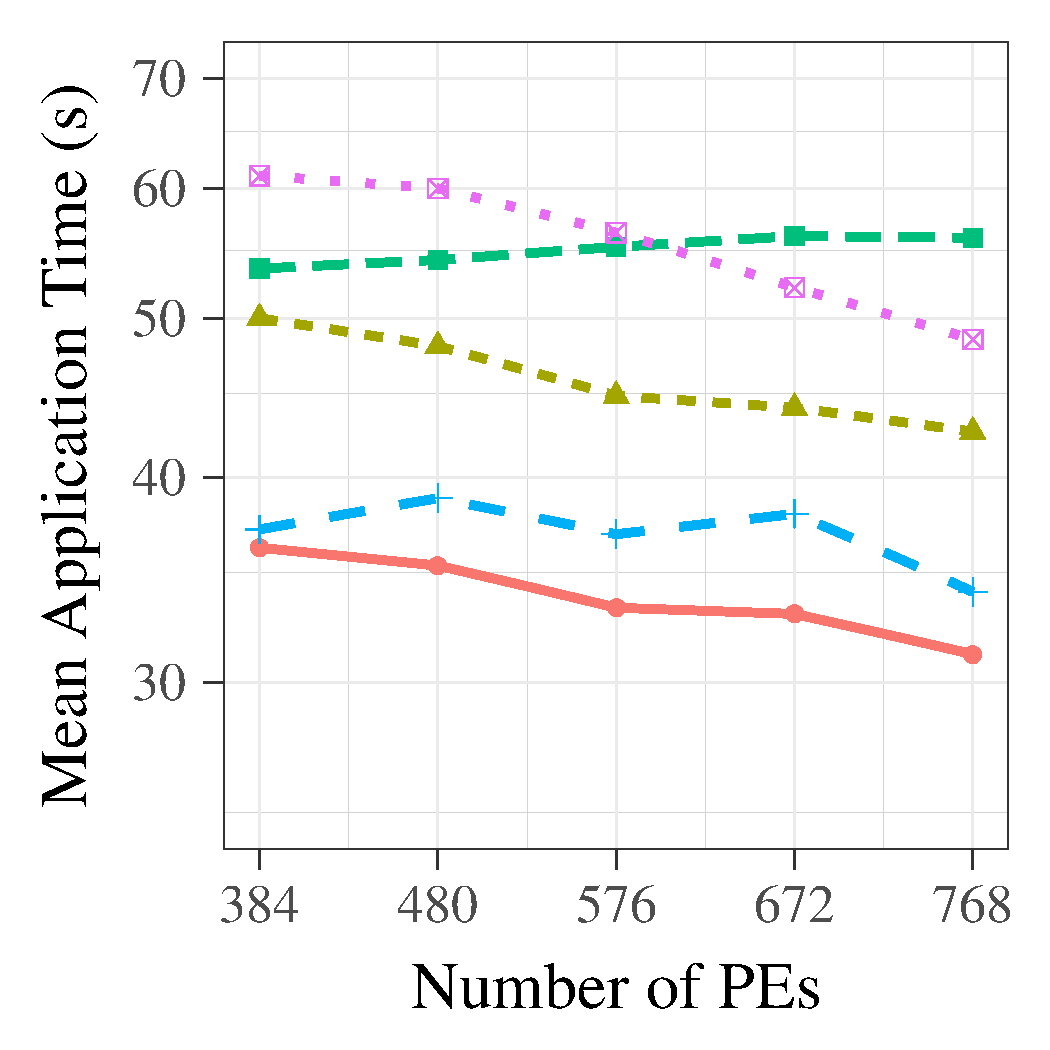
\includegraphics[width=0.49\linewidth]{images/apptime_leanmd_sdumont_log.pdf}\label{fig:eval:sdumont:leanmd:apptime}}
 \subfigure[Rescheduling Time (s).]{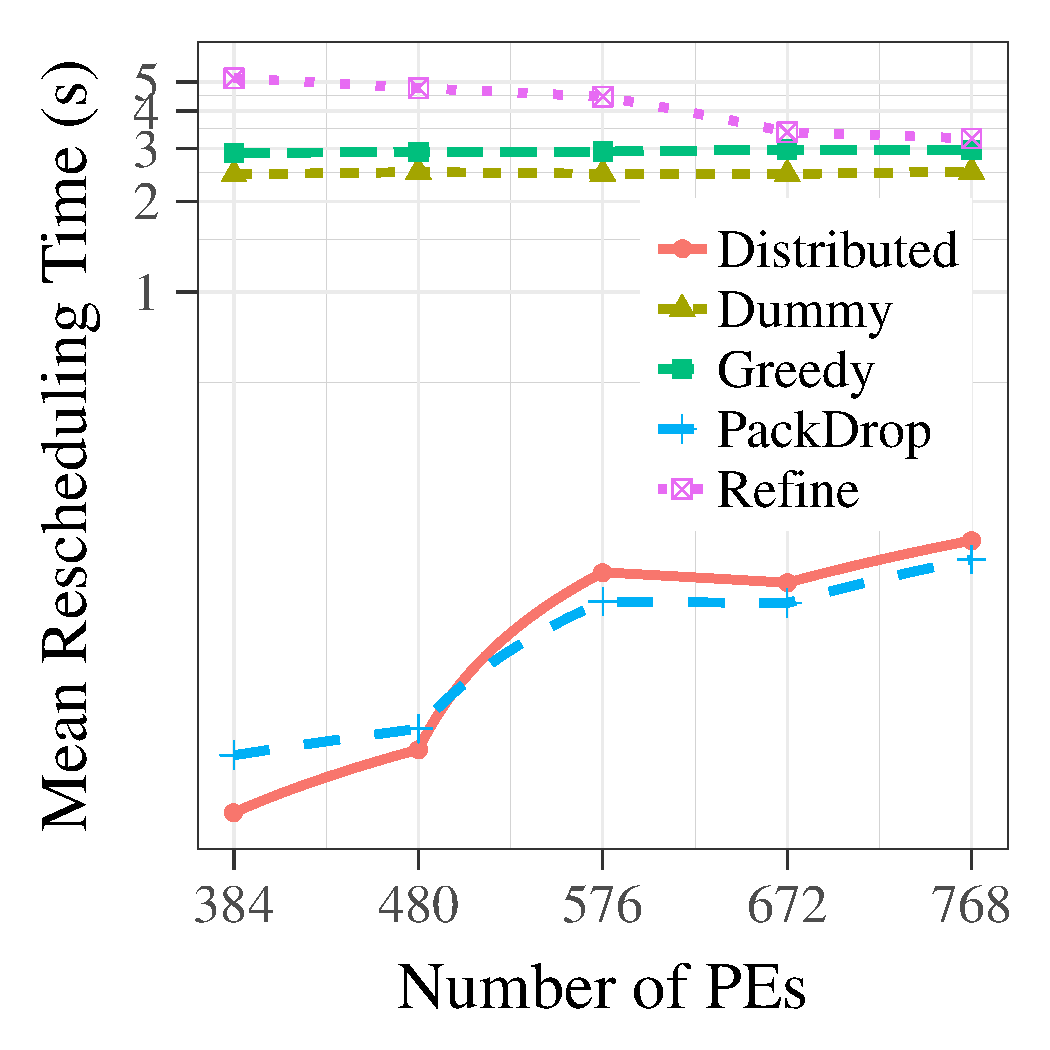
\includegraphics[width=0.49\linewidth]{images/schedtime_leanmd_sdumont_log.pdf}\label{fig:eval:sdumont:leanmd:schedtime}}
 \caption{\textit{LeanMD} execution results on Platform 2.}
 \label{fig:eval:sdumont:leanmd}
\end{figure}

%\begin{figure}[!ht]
% \centering
% 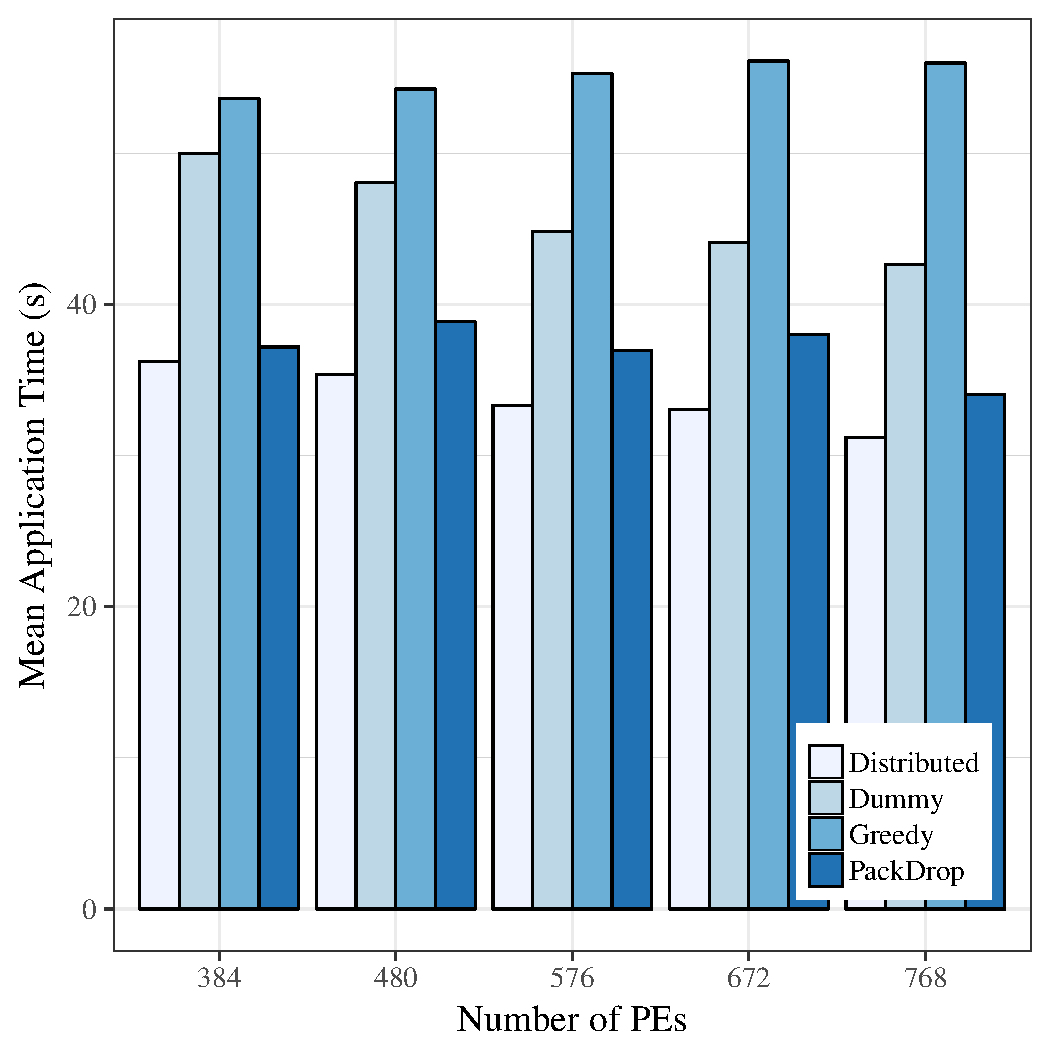
\includegraphics[width=0.9\linewidth]{images/apptime_leanmd_sdumont_bars.pdf}
% \caption{LeanMD supercomputer AppTime execution results.}
% \label{fig:eval:sdumont:leanmd:apptime:bars}
%\end{figure}

%\begin{figure}
%	\centering
%	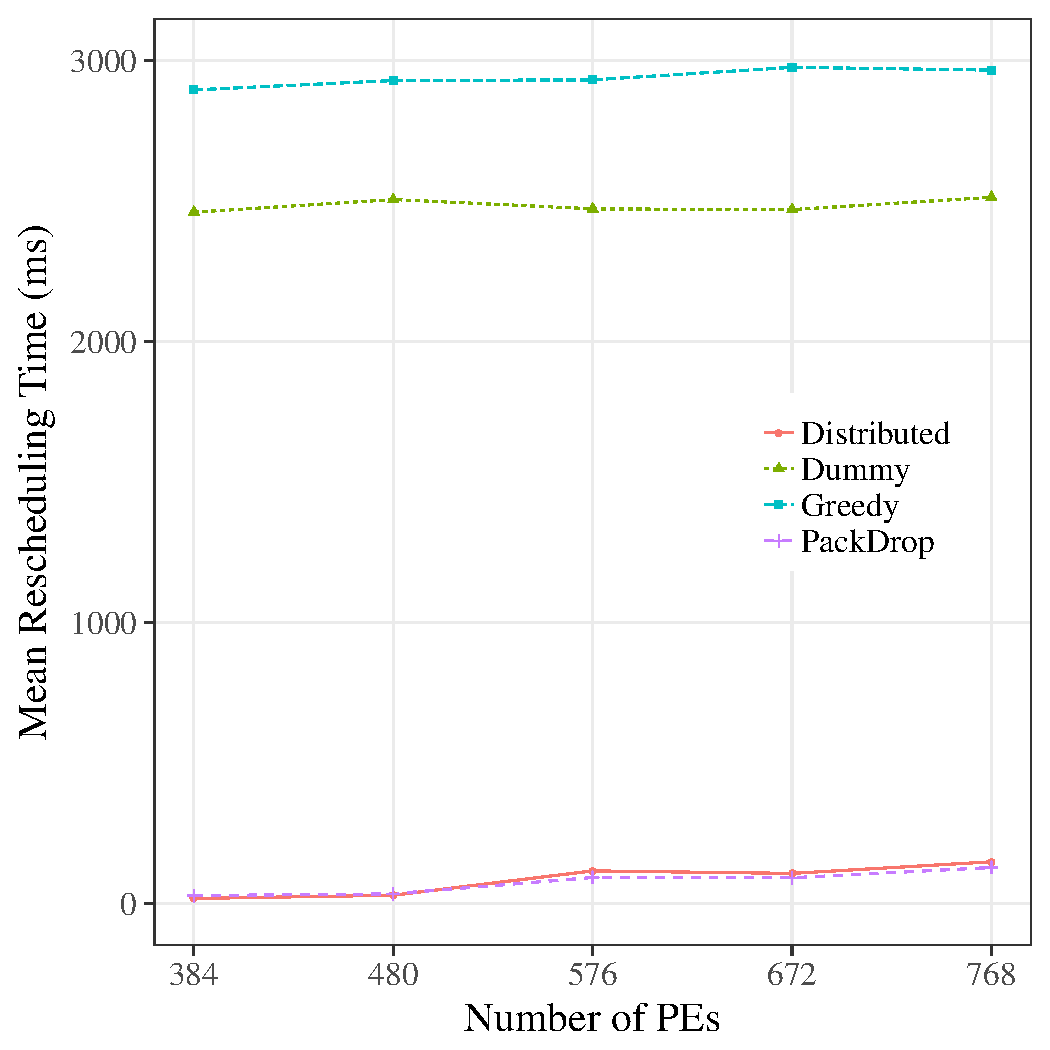
\includegraphics[width=0.9\linewidth]{images/schedtime_leanmd_sdumont.pdf}
%	\caption{LeanMD supercomputer SchedTime execution results.}
%	\label{fig:eval:sdumont:leanmd:schedtime}
%\end{figure}

Results of mean application time are displayed in Figure~\ref{fig:eval:sdumont:leanmd:apptime} and mean rescheduling time in Figure~\ref{fig:eval:sdumont:leanmd:schedtime}, both in a $log$ scale to better exhibit the differences between \distributedlb and \packdrop.
%\refinelb was excluded from this evaluation since \textit{LeanMD} input presents more data than \refinelb is able to process in a reasonable time, being on average $1,000$ms slower than \greedylb in the $384$ PEs test case. % Nenhuma ideia de tempo geral? O que é razoável?
In this evaluation, \refinelb had a very low efficiency, being $1$s slower than \greedylb in the $384$ PEs scenario.
It was able to perform better as PE numbers grew, but was ultimately unable to compete with distributed approaches.

\distributedlb benefits from this platform due to Infiniband's low latency communication costs, which reflects on improved total application times, as seen in Figure~\ref{fig:eval:sdumont:leanmd:apptime}.
\packdrop followed it closely and we can see that its rescheduling time in larger systems outperforms \distributedlb, displayed in Figure~\ref{fig:eval:sdumont:leanmd:schedtime}.

The rescheduling and application time results of \textit{LeanMD} in this platform highlight the importance of using scalable approaches to balance system load, as well as using available parallelism in execution environments.
This is specially visible in \greedylb results on Figure~\ref{fig:eval:sdumont:leanmd:apptime}, where the application performance was decreased after the global rescheduling process.
Increased migration costs and higher \textit{hop} counts in communication, consequences of load balancing, heavily impacted \textit{LeanMD} in this case.

\subsection{Performance Evaluation Overview} \label{eval:overview}

Most scientific applications today seek strong scaling, increasing their computational platforms to solve problems faster.
Our results showed that, to achieve such an objective, an application must implement efficient load balancing strategies.
We presented \packdrop as a solution for scalable rescheduling of work in distributed memory systems.

Section~\ref{sec:cluster:lbtest} showed that \packdrop is able to effectively balance the load. 
Results highlight the importance of load balancing even in synthetic loads.
The \textit{LB Test} benchmark used has very low migration and communication overhead, and most of its work is done locally, which is optimal for rescheduling evaluation of raw computational workload.
Moreover, \textit{LB Test} is known for having a very low migration cost and simple tasks, which enhances the effectiveness of centralized approaches such as \refinelb.
These results also portray the addition of communication overheads in different topologies ($2$, $4$, and $6$ communication edges for Ring, Mesh2D, and Mesh3D, respectively). %Can I use peers here?
As communication affects the application time more, migrations impact the total application time more, as we can see in the \greedylb results.

%Our strategy was only outperformed by \tofix{\textit{Refine} in all test cases, which is expected, since the total load dealt with is considerably small ($\sim 19$K tasks) and migrations cheap, which benefits centralized schedulers.}

In Sections~\ref{sec:cluster:md}~and~\ref{sec:sdumont:md}, we evaluated \packdrop in \textit{LeanMD} (better described in Section~\ref{sec:benchmarks}).
This represents ``a real world-like" scenario, in which applications may have dynamic communication patterns and high migration overhead.
Results presented here highlight the overhead of centralized rescheduling approaches when joined with large-scale applications ($171$K tasks) and big environments, which increases work and information aggregation costs, respectively.

\distributedlb outperformed our approach in Platform 2, due to its more refined take on load balancing and high-speed network interconnection.
However, the results show that \packdrop and its locality friendly batching of tasks for migration guarantees better performance in Platform 1, which portrays a Gigabit Ethernet interconnection.
Finally, \packdrop was able to efficiently scale applications among all observed platforms, and had a faster rescheduling time than \distributedlb in most of the observed cases.
